\documentclass{article}
\usepackage{graphicx}
\usepackage{sidecap}
\title{Cpppc Project: Microfluidic-Large-Scale-Integration (mLSI) Simulator}
\author{Mengchu Li}
\begin{document}
\maketitle
\section{Introduction}

Microfluidic Large-Scale Integration (mLSI) is a promising platform for biological/biochemical applications. An mLSI chip has a multi-layered structure consisting of micro-channels and micro-mechanical valves. The flow layer is responsible for fluid transportation and operation execution, and the control layer is responsible for valve actuation that manipulates the direction of the fluid-flow.  
Figure~\ref{fig:mlsi} shows a photo of an mLSI chip where control channels are filled with green food dye and flow channels are filled with red food dye.

MLSI is a developing research filed. Currently there is no simulation tool that can predicts the flow status on an mLSI chip. Different from existing microfluidic simulators, the main objective of which is to accurately predict the movement of small fluid particles, mLSI simulation should focus on the correlating valves and channels. More specifically, it should predict the channel status, i.e. whether a channel is blocked, vacant, or filled with fluids at a specific time point. In other world, mLSI simulation predicts the fluid behavior on a system-level.

\begin{SCfigure}
\caption{An mLSI chip for kinase activity applications.}
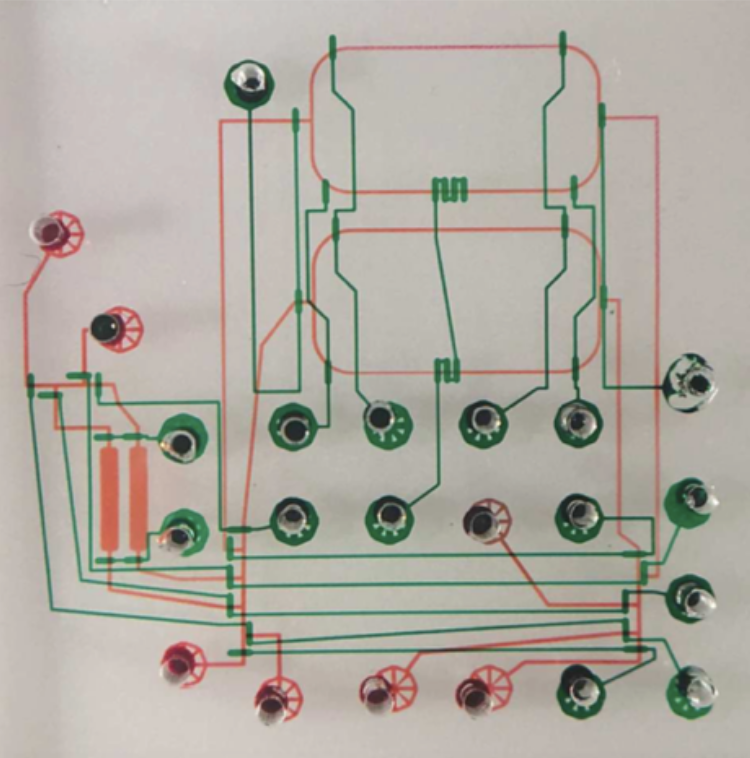
\includegraphics[height = 5cm]{mlsi}
\label{fig:mlsi}
\end{SCfigure}

\section{Overview of the Project}
This project aims to develop a prototype of mLSI simulator. Formally:
\paragraph{Input}
\begin{itemize}
\item A description of the physical structure of an mLSI chip (.txt file);
\item A description of the application protocols (txt.file);
\item A specific time point (a floating point number).
\end{itemize}
\paragraph{Output}
\begin{itemize}
\item The channel status, i.e. whether it is blocked, vacant or filled with fluids, at a specific time point (txt.file).
\end{itemize}

\begin{figure}
\caption{System diagram of the Project}
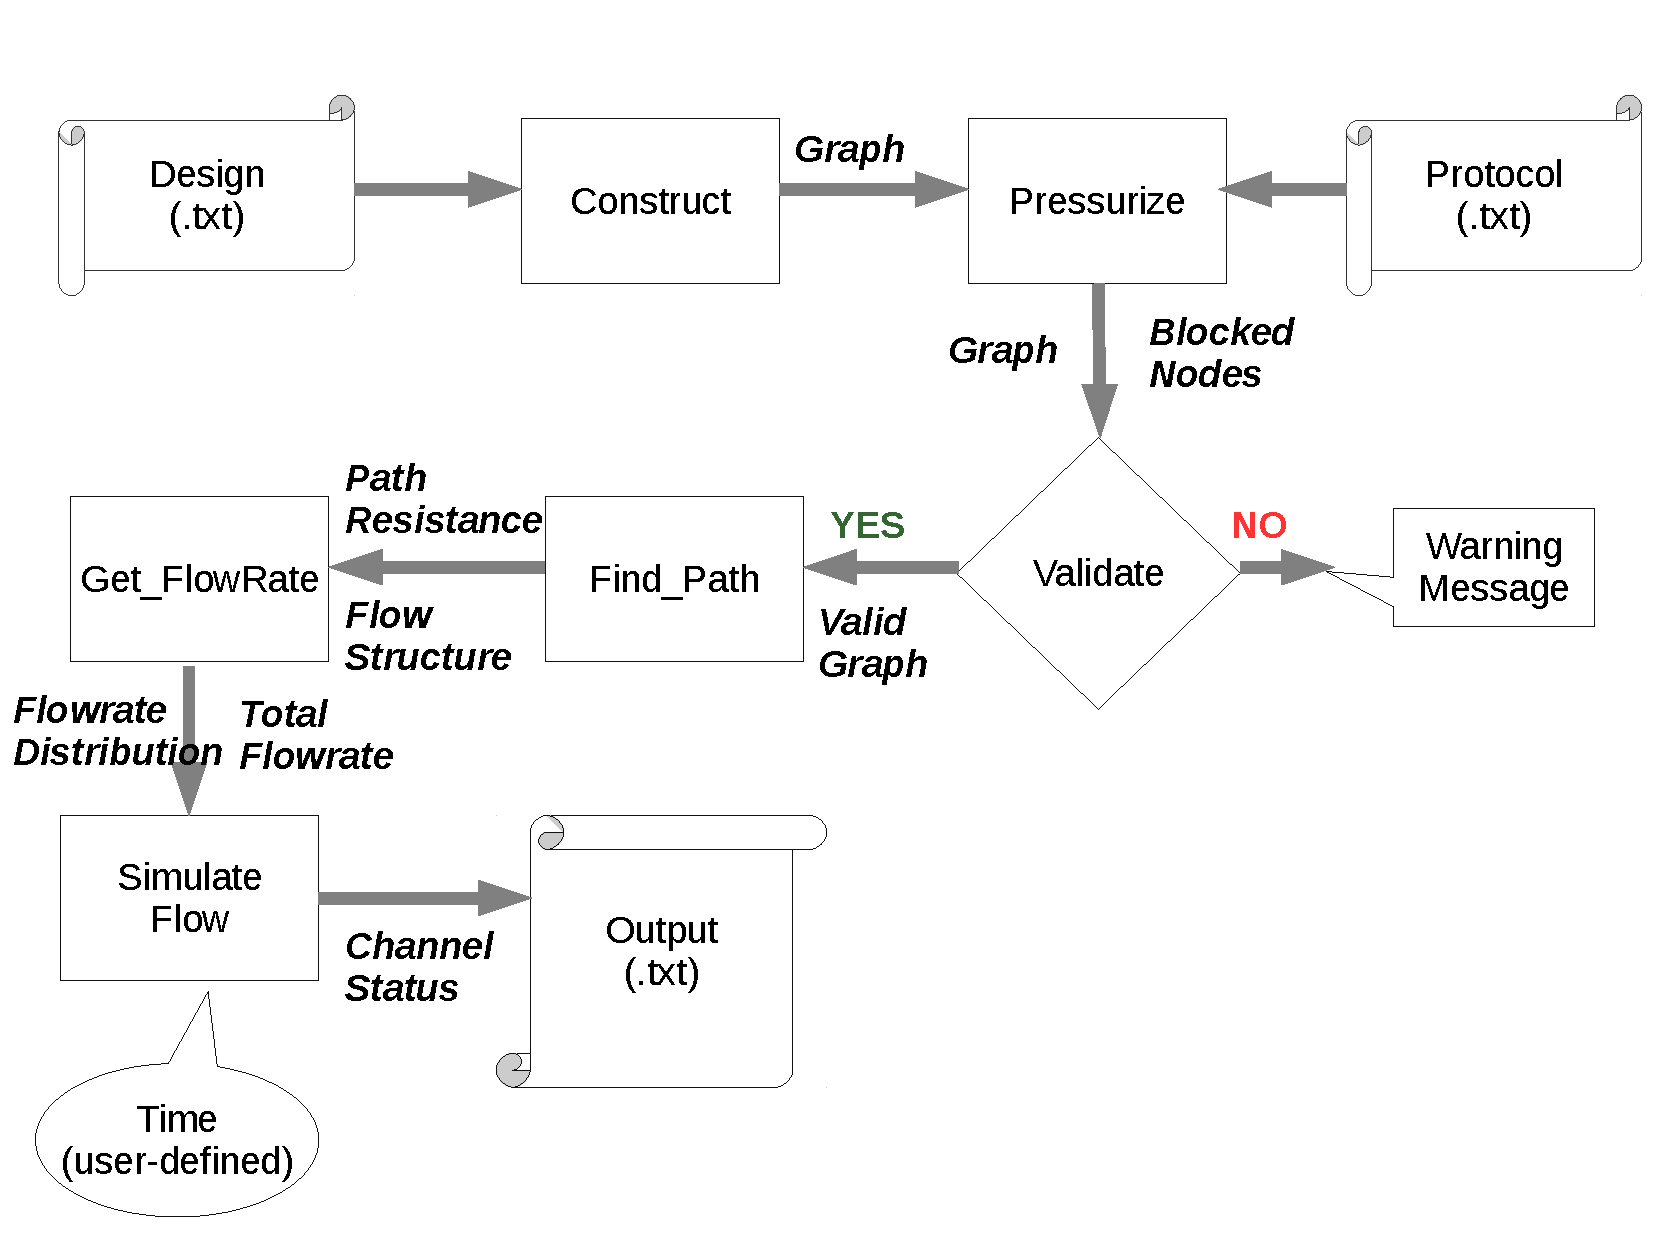
\includegraphics[height = 8cm]{systemdiagram}
\label{fig:system}
\end{figure}

Figure~\ref{fig:system} shows the system diagram of the simulator. 
The simulator first takes a description of the chip \textit{design} as its input, and \textit{constructs} a \textbf{graph} structure consisting of nodes and edges. Each node may represent an inlet, an outlet, a valve, or a channel branching point of the mLSI chip, and each edge represents a channel segment that connects two nodes.
After that, the simulator reads a description of application \textit{protocols},
based on which some of the control channels will be \textit{pressurize}d,
and thus some nodes will be blocked.
The \textbf{graph} and the \textbf{blocked nodes} are then fed to the next process that \textit{validate}s whether there is any feasible flow paths on the chip.
If there is no feasible flow path, the simulator will output a \textit{warning message} and terminate. If there is one or more feasible flow paths, the simulator will generate a \textbf{valid graph} where blocked nodes and channels are removed. 

\end{document}